%%%%%%%%%%%%%%%%%%%%%%%%%%%%%%%%%%%%%%%%%

% LaTeX Template for IAHR YPN Congress

%%%%%%%%%%%%%%%%%%%%%%%%%%%%%%%%%%%%%%%%%

%----------------------------------------------------------------------------------------
%	PACKAGES AND OTHER DOCUMENT CONFIGURATIONS
%----------------------------------------------------------------------------------------

\documentclass[landscape,a1paper,fontscale=0.45]{baposter} % Adjust the font scale/size here

\usepackage{graphicx} % Required for including images
\graphicspath{{images/}} % Directory in which figures are stored

\usepackage{hyperref}
\hypersetup{colorlinks, citecolor=blue, filecolor=blue, linkcolor=blue, urlcolor=blue}

\usepackage{amsmath} % For typesetting math
\usepackage{amssymb} % Adds new symbols to be used in math mode

\usepackage{booktabs} % Top and bottom rules for tables
\usepackage{enumitem} % Used to reduce itemize/enumerate spacing
\usepackage{palatino} % Use the Palatino font
\usepackage[font=small,labelfont=bf]{caption} % Required for specifying captions to tables and figures

\usepackage{multicol} % Required for multiple columns
\setlength{\columnsep}{1em} % Slightly increase the space between columns
\setlength{\columnseprule}{0mm} % No horizontal rule between columns

\usepackage{tikz} % Required for flow chart
\usetikzlibrary{shapes,arrows} % Tikz libraries required for the flow chart in the template
\usepackage{paracol}

\newcommand{\compresslist}{ % Define a command to reduce spacing within itemize/enumerate environments, this is used right after \begin{itemize} or \begin{enumerate}
\setlength{\itemsep}{1pt}
\setlength{\parskip}{0pt}
\setlength{\parsep}{0pt}
}

\definecolor{lightblue}{rgb}{0.145,0.6666,1} % Defines the color used for content box headers

\begin{document}

\begin{poster}
{
headerborder=closed, % Adds a border around the header of content boxes
colspacing=1em, % Column spacing
bgColorOne=white, % Background color for the gradient on the left side of the poster
bgColorTwo=white, % Background color for the gradient on the right side of the poster
borderColor=lightblue, % Border color
headerColorOne=black, % Background color for the header in the content boxes (left side)
headerColorTwo=lightblue, % Background color for the header in the content boxes (right side)
headerFontColor=white, % Text color for the header text in the content boxes
boxColorOne=white, % Background color of the content boxes
textborder=roundedleft, % Format of the border around content boxes, can be: none, bars, coils, triangles, rectangle, rounded, roundedsmall, roundedright or faded
eyecatcher=true, % Set to false for ignoring the left logo in the title and move the title left
headerheight=0.1\textheight, % Height of the header
headershape=roundedright, % Specify the rounded corner in the content box headers, can be: rectangle, small-rounded, roundedright, roundedleft or rounded
headerfont=\Large\bf\textsc, % Large, bold and sans serif font in the headers of content boxes
%textfont={\setlength{\parindent}{1.5em}}, % Uncomment for paragraph indentation
linewidth=2pt % Width of the border lines around content boxes
}
%----------------------------------------------------------------------------------------
%	TITLE SECTION 
%----------------------------------------------------------------------------------------
%
{
\includegraphics[height=6em]{images/logo_white.png}} % First university/lab logo on the left
{\bf\textsc{Metoda trójwymiarowego modelowania obszarów urbanistycznych z wykorzystaniem metod fotogrametrii}\vspace{0.5em}} % Poster title
{\textsc{Daniel Borkowski, Julia Farganus, Rafał Mielniczuk, Katarzyna Wochal, promotor Marek Krótkiewicz}}
% Author names and institution
{
\includegraphics[height=6em]{images/zpi-logo.png}} % Second university/lab logo on the right

%----------------------------------------------------------------------------------------
%	ABSTRACT
%----------------------------------------------------------------------------------------

\headerbox{Abstrakt}{name=abstract,column=0,span=2, row=0}{

\begin{center}
    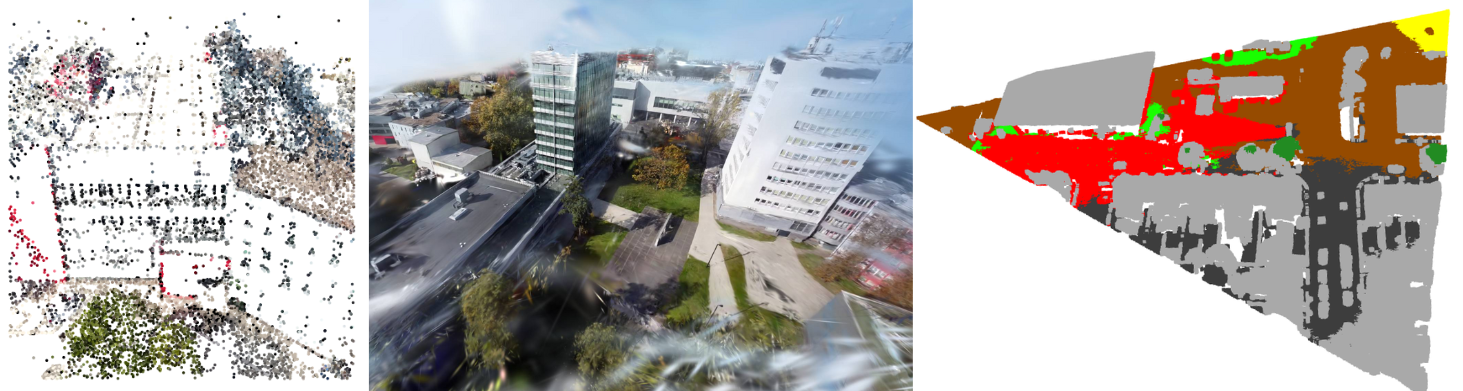
\includegraphics[width=0.9\linewidth]{images/kolaz.png}
\end{center}

Projekt obejmował stworzenie aplikacji do modelowania trójwymiarowych scen miejskich na podstawie zdjęć fotogrametrycznych, wykorzystującej metody \textit{structure from motion} i \textit{gaussian splatting} oraz segmentację semantyczną. % Dzięki integracji zaawansowanych rozwiązań i efektywnemu procesowi \textit{end-to-end}, aplikacja ma potencjał zastosowań w takich branżach jak gry wideo, architektura, robotyka, pojazdy autonomiczne i urbanistyka.

\vspace{0.6em}

\textbf{Słowa kluczowe:} reconstruction, 3D modeling, urban modeling, semantic segmentation, gaussian splatting.

\vspace{0.3em} % When there are two boxes, some whitespace may need to be added if the one on the right has more content
}

%----------------------------------------------------------------------------------------
%	AKWIZYCJA & REKONSTRUKCJA
%----------------------------------------------------------------------------------------

\headerbox{Akwizycja i rekonstrukcja}{name=akwizycja_rekonstrukcja,column=0, span=2, below=abstract}{

\begin{multicols}{2}
W projekcie zastosowano metody fotogrametryczne do pozyskania zdjęć z drona i gruntu na terenie Politechniki Wrocławskiej, obejmujących budynki \textbf{C5}, \textbf{C7} oraz \textbf{Strefę Kultury Studenckiej}. Zdjęcia wykonano z wielu kątów, zapewniając odpowiednie nakładanie się ujęć do poprawnej rekonstrukcji 3D. Następnie, przy użyciu techniki \textbf{Structure from Motion} (SfM), wygenerowano chmurę punktów 3D, określając rozmieszczenie punktów w przestrzeni oraz pozycje i orientacje kamer. Uzyskana chmura punktów została dodatkowo poddana filtracji z wykorzystaniem metod opartych na ana\mbox{lizie} sąsiedztwa każdego punktu.

\begin{center}
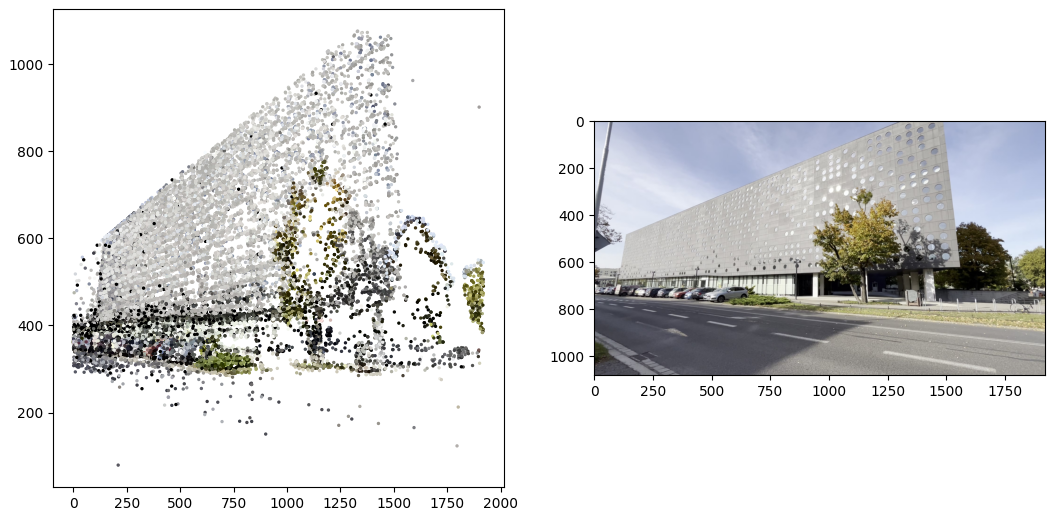
\includegraphics[width=1\linewidth]{images/sfm-c.png}
\captionof{figure}{Projekcja przykładowej chmury punktów na płaszczyznę porównana do zdjęcia}
\end{center}

\end{multicols}
}


%----------------------------------------------------------------------------------------
%	FLOW
%----------------------------------------------------------------------------------------

\headerbox{Przebieg procesu}
{name=flow,column=2,span=2, row=0}{ % This block is as tall as the references block

\begin{center}
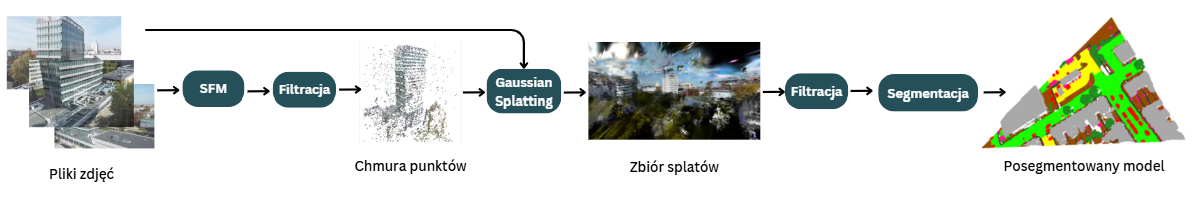
\includegraphics[width=1\linewidth]{images/przebieg.png}
\captionof{figure}{Diagram pokazujący kolejne etapy procesu wraz z danymi wejściowymi i wyjściowymi}
\end{center}

}


%----------------------------------------------------------------------------------------
%	GAUSSIAN SPLATTING
%----------------------------------------------------------------------------------------

\headerbox{Gaussian Splatting}{name=gaussian_splatting,column=2,span=2,below=flow}{

\begin{multicols}{2}

Wykorzystano bibliotekę \textit{gsplat} do testowania różnych hiperparametrów algorytmu \textbf{Gaussian Splatting}, optymalizując trenowanie pod względem czasu i pamięci. Kluczowe były liczba gaussianów, strategia i częstość adaptacji, liczba iteracji i stopień zmiennych harmonicznych.

\begin{center}
\begin{tabular}{l l l l l l}
\toprule
\textbf{scena} & \textbf{PSNR} & \textbf{LPIPS} & \textbf{SSIM} & \textbf{LG} & \textbf{Czas} \\
\midrule
SKS & 22.03 & 0.71 & 0.25 & 2,9\text{e+}6 & 2:53 \\
C5 & 21.98 & 0.71 & 0.26 & 4,5\text{e+}6 & 10:40 \\
C7 & 22.63 & 0.72 & 0.29 & 3,0\text{e+}6 & 15:15 \\
\bottomrule
\end{tabular}
\captionof{table}{Metryki PSNR, SSIM oraz LPIPS, liczba gaussianów oraz czas trenowania dla testowych scen.}
\end{center}

\begin{center}
    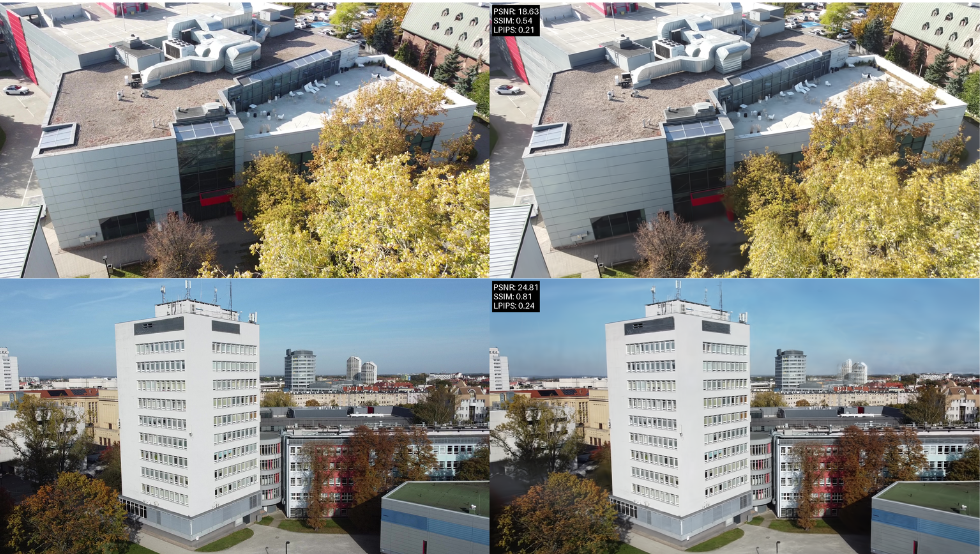
\includegraphics[width=0.9\linewidth]{images/gs-examples.png}
    \captionof{figure}{Przykładowe wizualizacje dla SKS oraz C5 (od lewej do prawej: prawdziwe zdjęcie i widok modelu)}
\end{center}

\end{multicols}

%------------------------------------------------

}

%----------------------------------------------------------------------------------------
%	PODSUMOWANIE
%----------------------------------------------------------------------------------------

\headerbox{Podsumowanie}{name=block,column=0,span=2,above=bottom}{ % This block is as tall as the references block
Opracowane oprogramowanie umożliwia kompleksowe modelowania obszarów miejskich z wykorzystaniem fotogrametrii. Wśród oferowanych użytkownikowi funkcjonalności znajdują się m.in. dostosowywanie parametrów, wczytywanie zdjęć, uruchamianie poszczególnych etapów oraz przeglądanie rezultatów. Odpowiednio dobrane i dostrojone algorytmy zapewniają jakościowe wyniki, które mogą być wykorzystywane razem lub oddzielnie.


}


%----------------------------------------------------------------------------------------
%	SEGMENTACJA
%----------------------------------------------------------------------------------------

\headerbox{Segmentacja}{name=segmentacja,column=2,span=2,below=gaussian_splatting,bottomaligned=block}{

\begin{multicols}{2}
\vspace{1em}
Przeprowadzono segmentację semantyczną chmury punktów, przypisując każdemu punktowi kategorię, taką jak budynek, droga czy zieleń miejska. Wykorzystano do tego implementację sieci \textbf{PointNet} w bibliotece \textit{Pytorch} oraz zbiór danych SensatUrban. Kluczowe wyzwania obejmowały próbkowanie danych, radzenie sobie z niezbalansowanymi kategoriami oraz unikanie wycieku danych, co rozwiązano m.in. przez ważenie funkcji straty i odpowiednie przygotowanie zestawów treningowych. Poprzez podział wejściowej chmury na tzw. \textit{chunki} model jest w stanie przeprowadzić inferencję na zbiorze punktów o wielkości nawet paru milionów elementów.

\begin{center}
\begin{tabular}{l l l}
\toprule
\textbf{Metryki} & \textbf{Unweighted Model} & \textbf{Weighted Model}  \\
\midrule
OwA & 43 & 51 \\
OwF & 38 & 46 \\
budynkiF & 87 & 84 \\
zieleńF & 0 & 42 \\
\bottomrule
\end{tabular}
\captionof{table}{Metryki: średnia ważona dokładność, średni ważony F1-score, F1-score dla klas: budynki i zieleń miejska}
\end{center}

\begin{center}
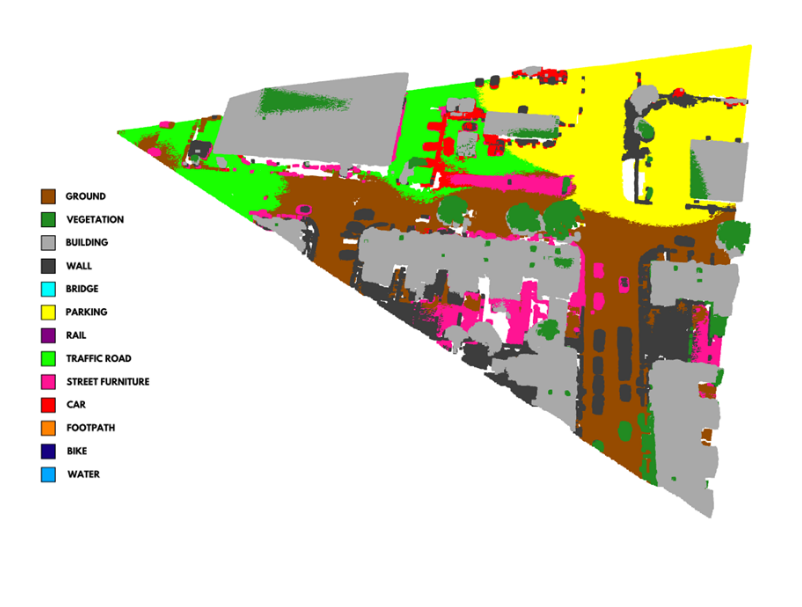
\includegraphics[width=1\linewidth]{"images/SFM (4).png"}
\captionof{figure}{Segmentacja na jednym z bloków ze zbioru SensatUrban}
\end{center}

\end{multicols}
}
%----------------------------------------------------------------------------------------
%	RENDEROWANIE
%----------------------------------------------------------------------------------------

\headerbox{Renderowanie}{name=rendering,column=0, span=2,below=akwizycja_rekonstrukcja,above=block}{ % This block's bottom aligns with the bottom of the conclusion block

\begin{multicols}{2}
    
    Zaprojektowano intuicyjny interfejs w \textit{PyQt} i \textit{QML}, zintegrowany z wydajnym systemem renderowania \textit{GPU} opartym na \textit{OpenGL}, \textit{OpenCL} i języku \textit{C}, oferującym także wsparcie dla \textit{VisPy}. Aplikacja zapewnia spójne środowisko do obsługi modeli 3D, obejmujące procesy takie jak generowanie chmury punktów, segmentacja i wizualizacja danych. Rendering wykorzystuje pliki .ply oraz Shader Storage Buffer Object (SSBO). Rysunek obok przedstawia główny widok aplikacji, w tym własny renderer.

    \begin{center}
    \includegraphics[width=0.85\linewidth]{images/"cloud-rendering.png"}
    \label{fig:renderer}
    \end{center}

\end{multicols}


}

%----------------------------------------------------------------------------------------
%	RESULTS 2
%----------------------------------------------------------------------------------------

% \headerbox{Results 2}{name=results2,column=1,below=abstract,bottomaligned=conclusion}{ % This block's bottom aligns with the bottom of the conclusion block

% Additional recommendations:
% \begin{itemize}\compresslist
%     \item Structure your poster by Abstract, Methods, Results and Conclusions. 
%     \item Every graphic/table should have a caption. 
%     \item Do not justify blocks of text on both sides.
%     \item Highlight your main finding. 
%     \item If possible, avoid abbreviations and acronyms. 
%     \item Where possible, express points as bullets rather than paragraphed text.
%     \item Use a constant font throughout the poster.
% \end{itemize}


% \textbf{Rule of thumb:}
% The poster is supposed to be readable in screen laptops. Check your final design in full screen.


% \begin{center}
% 
\includegraphics[width=0.6\linewidth]{placeholder.jpg}
% \captionof{figure}{Figure caption}
% \end{center}
% }

%----------------------------------------------------------------------------------------

\end{poster}

\end{document}